\section{Present results}

\begin{frame}
    \frametitle{Dam break}
    \begin{columns}[onlytextwidth]
        \begin{column}{0.5\textwidth}
            \begin{figure}[ht]
                \centering
                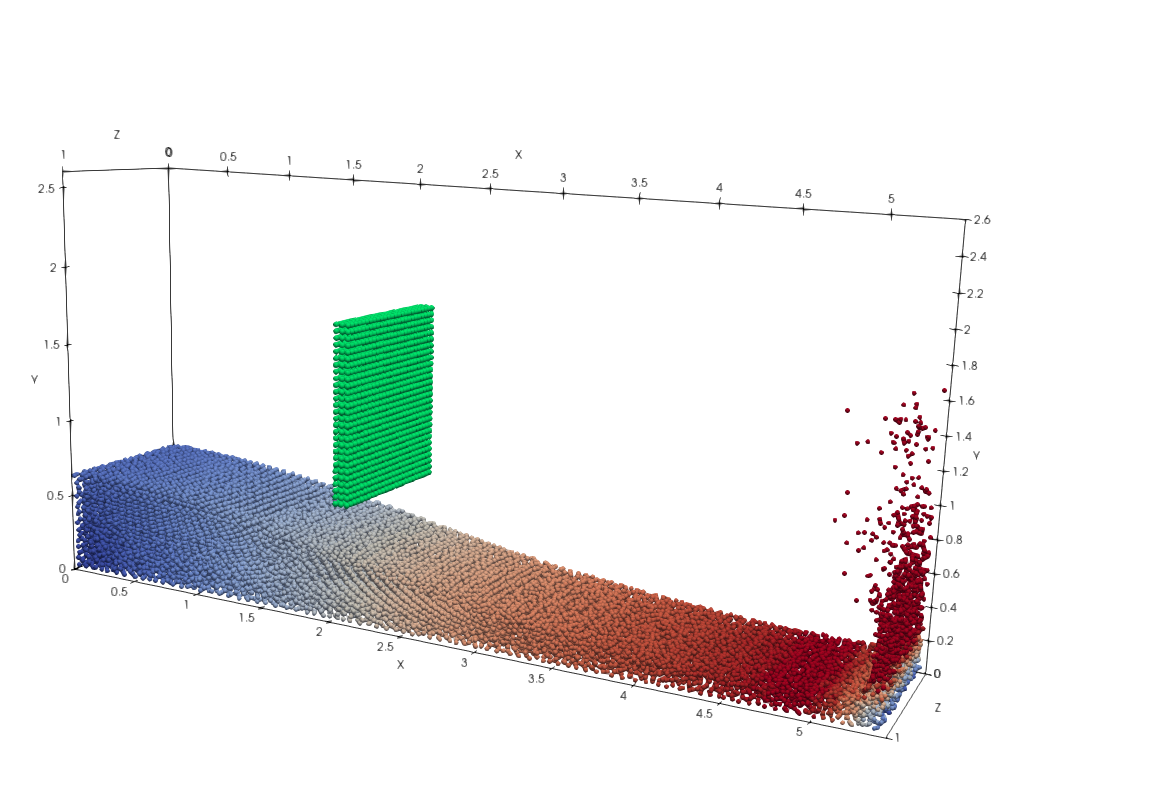
\includegraphics[width=\textwidth]{dam_break_3d}
                \caption{Free surface dam break with opening gate.}
            \end{figure}
        \end{column}
        \begin{column}{0.5\textwidth}
            \begin{figure}[ht]
                \centering
                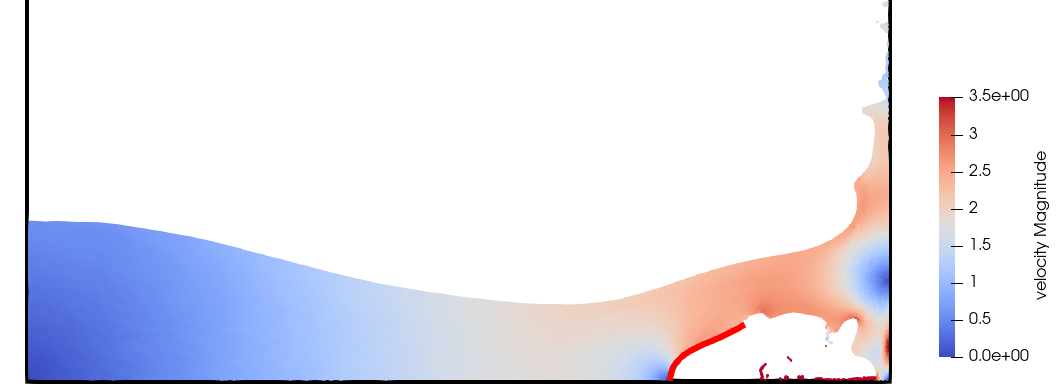
\includegraphics[width=\textwidth]{dam_break_gate_2d_b}
                \caption{Dam break impacting an elastic plate.}
            \end{figure}
        \end{column}
    \end{columns}
\end{frame}
\begin{frame}
    \frametitle{Falling spheres}
    \begin{columns}[onlytextwidth]
        \begin{column}{0.5\textwidth}
            \begin{figure}[ht]
                \centering
                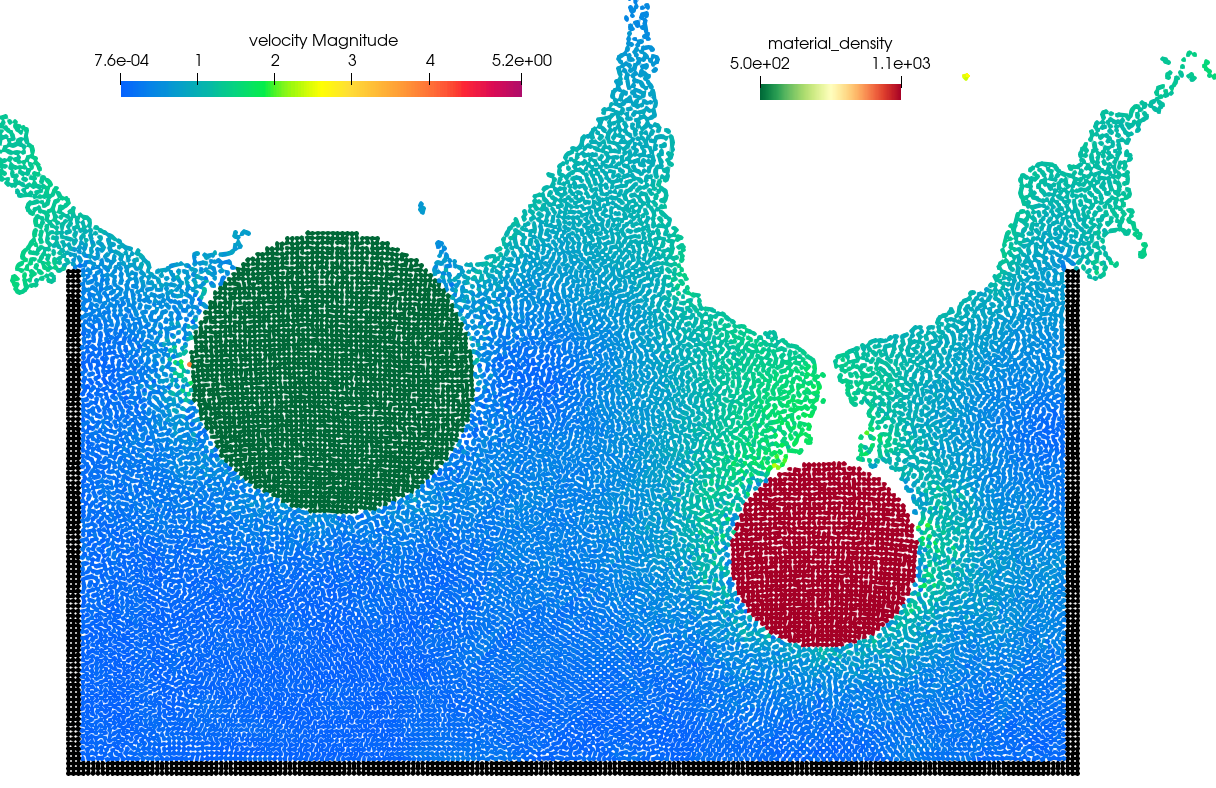
\includegraphics[width=0.8\textwidth]{falling_spheres_density}
                \caption{Two elastic spheres ($\rho_{\text{left}}=500$, $\rho_{\text{right}}=1100$) falling into a tank of water ($\rho_{\text{water}}=1000$).}
            \end{figure}
        \end{column}
        \begin{column}{0.5\textwidth}
            \begin{figure}[ht]
                \centering
                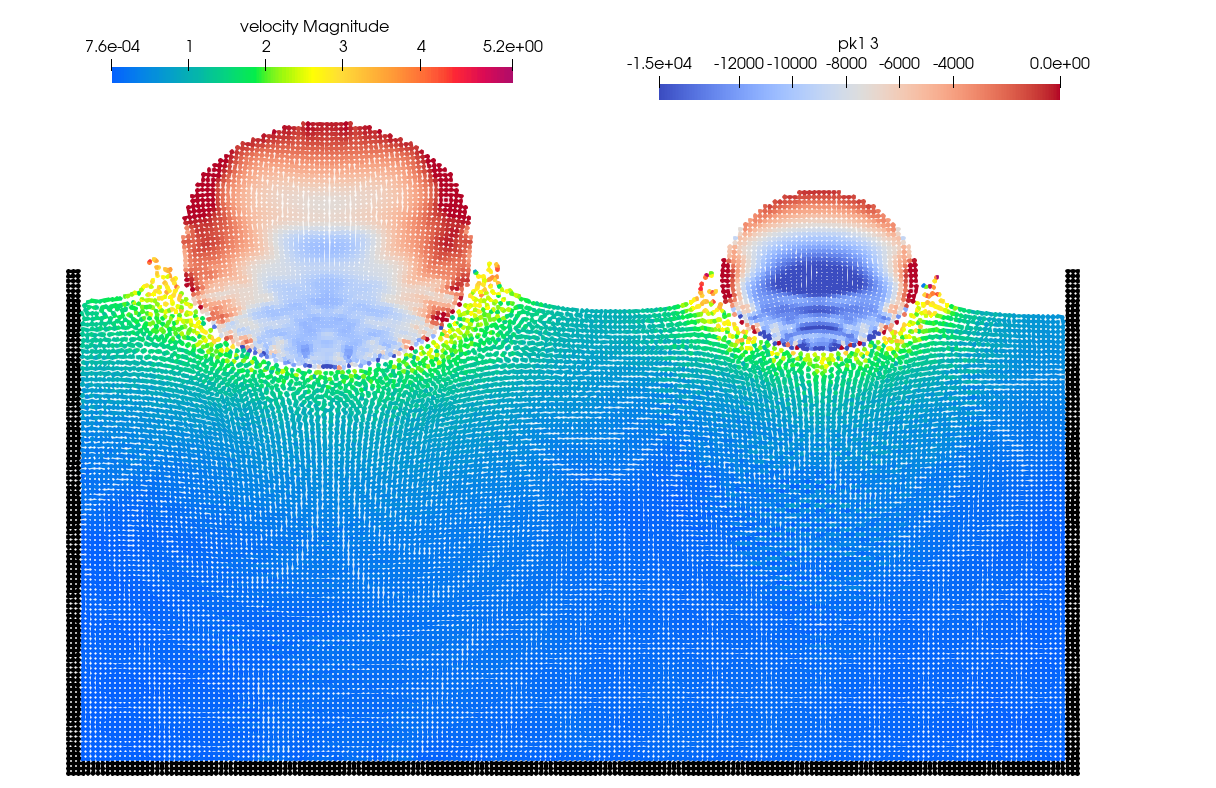
\includegraphics[width=0.8\textwidth]{falling_spheres_pk1}
                \caption{Pk1 stress tensor of elastic spheres.}
            \end{figure}
        \end{column}
    \end{columns}
\end{frame}
\begin{frame}
    \frametitle{Liquefied stanford bunny}
    \begin{columns}[onlytextwidth]
        \begin{column}{0.5\textwidth}
            \begin{figure}[ht]
                \centering
                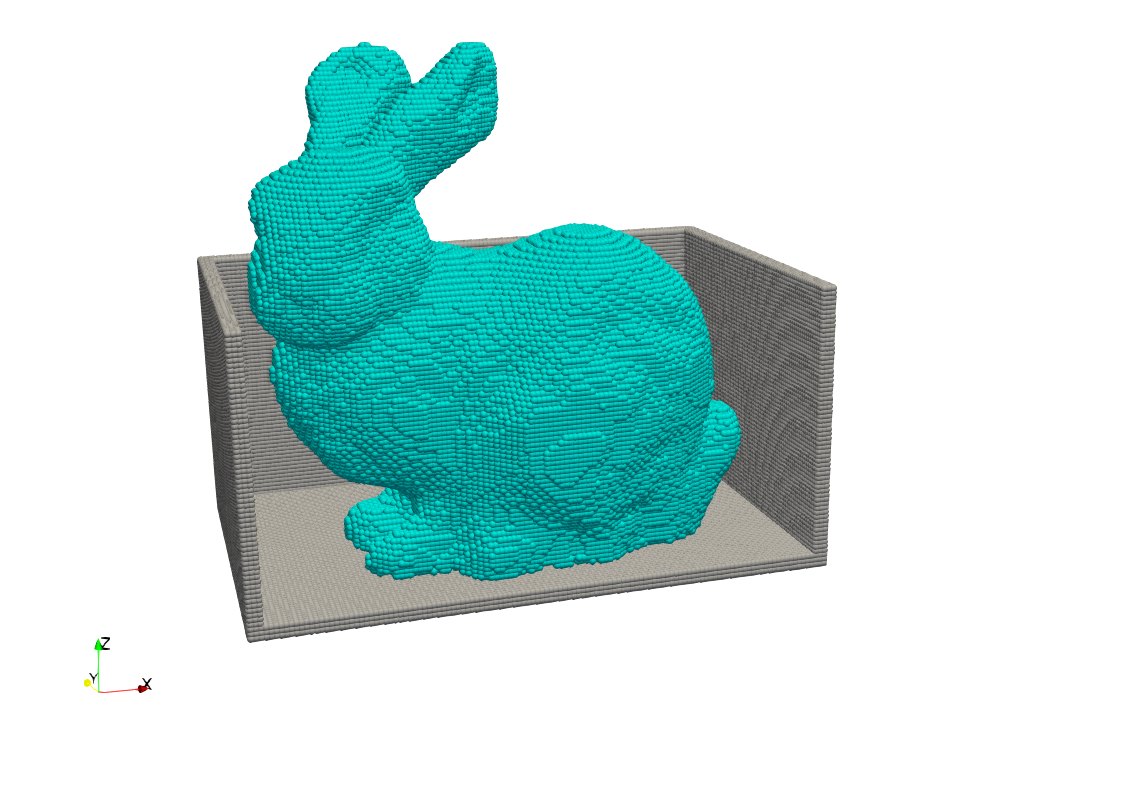
\includegraphics[width=\textwidth]{liquefied_bunny_1}
                \caption{At time $t = 0.0 \text{ sec}$}
            \end{figure}
        \end{column}
        \begin{column}{0.5\textwidth}
            \begin{figure}[ht]
                \centering
                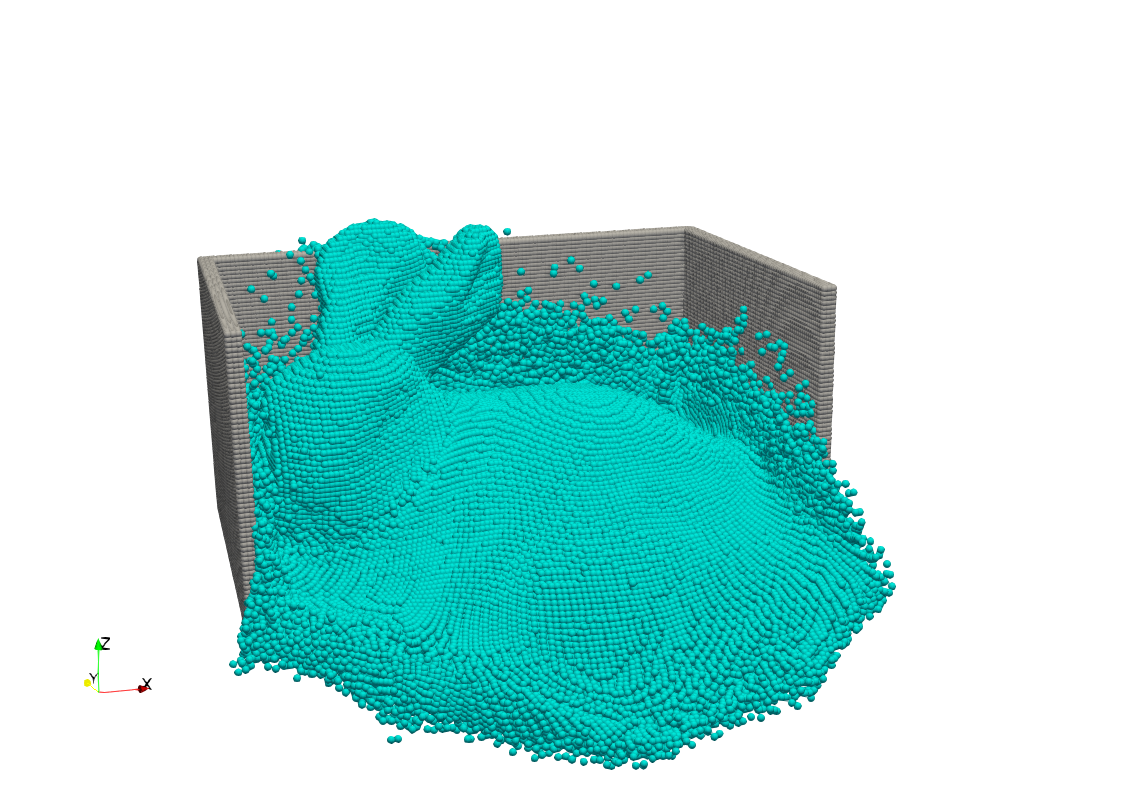
\includegraphics[width=\textwidth]{liquefied_bunny_2}
                \caption{At time $t = 0.6 \text{ sec}$}
            \end{figure}
        \end{column}
    \end{columns}
\end{frame}
\begin{frame}
    \frametitle{Others}
    \begin{columns}[onlytextwidth]
        \begin{column}{0.5\textwidth}
            \begin{figure}[ht]
                \centering
                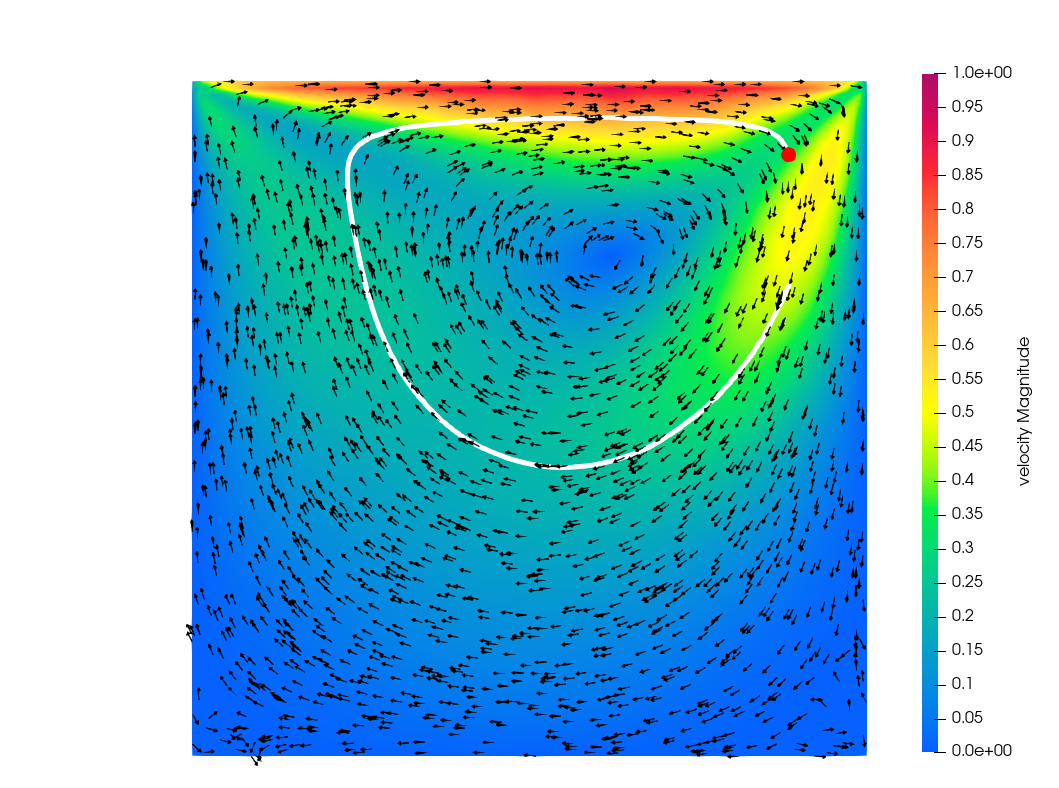
\includegraphics[width=\textwidth]{ldc}
                \caption{Lid driven cavity}
            \end{figure}
        \end{column}
        \begin{column}{0.5\textwidth}
            \begin{figure}[ht]
                \centering
                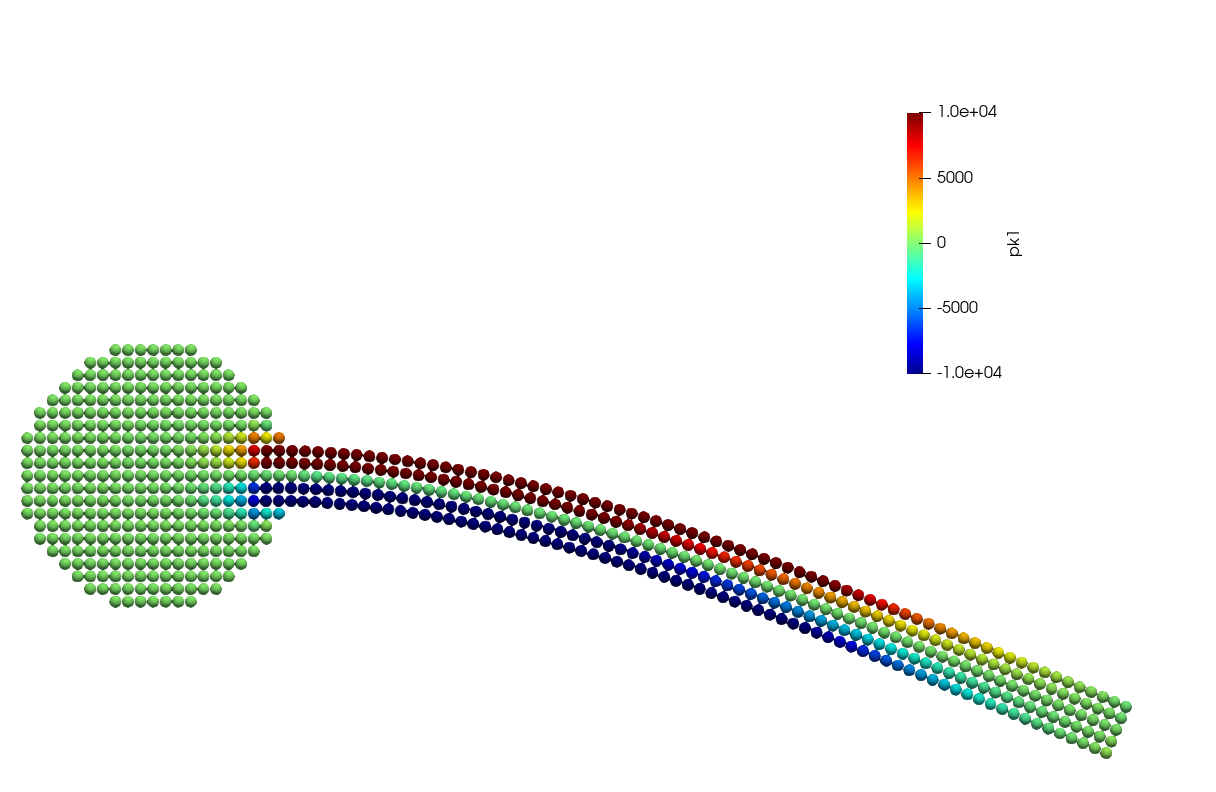
\includegraphics[width=\textwidth]{oscillating_beam}
                \caption{Oscillating beam}
            \end{figure}
        \end{column}
    \end{columns}
\end{frame}
